\mode*
\lecture[Introduction]{A Very Brief Internet Tutorial (I)}{intro}
\section{Introduction}

\subsection[Definition]{What's A Computer Network?}

\begin{frame}{{What's A Computer Network?}}
  \begin{center}
    \mode<beamer>{ 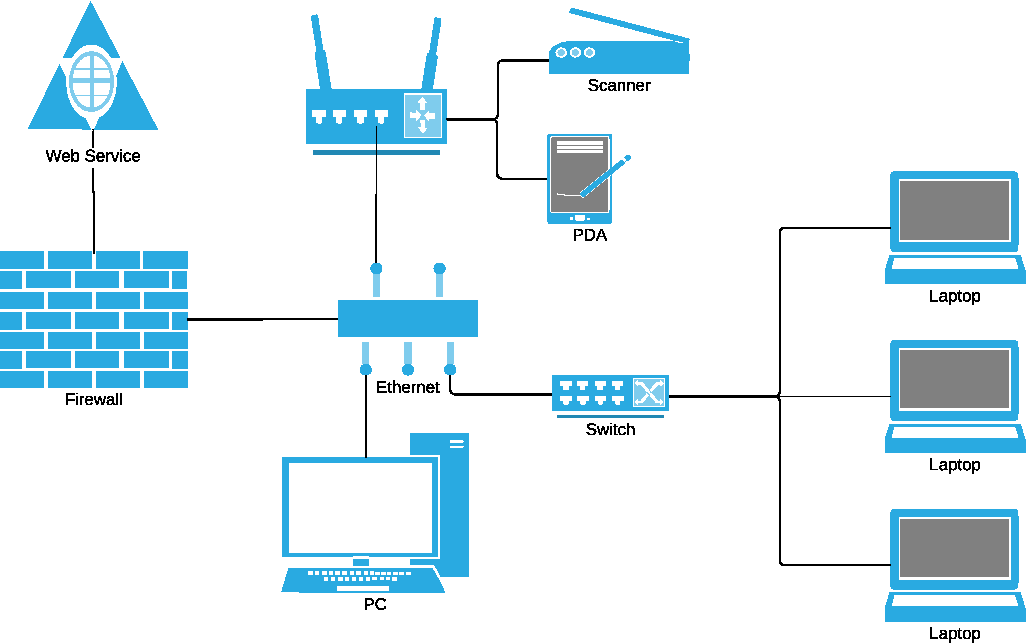
\includegraphics[width=.9\textwidth]{network} }%
    \mode<article>{ 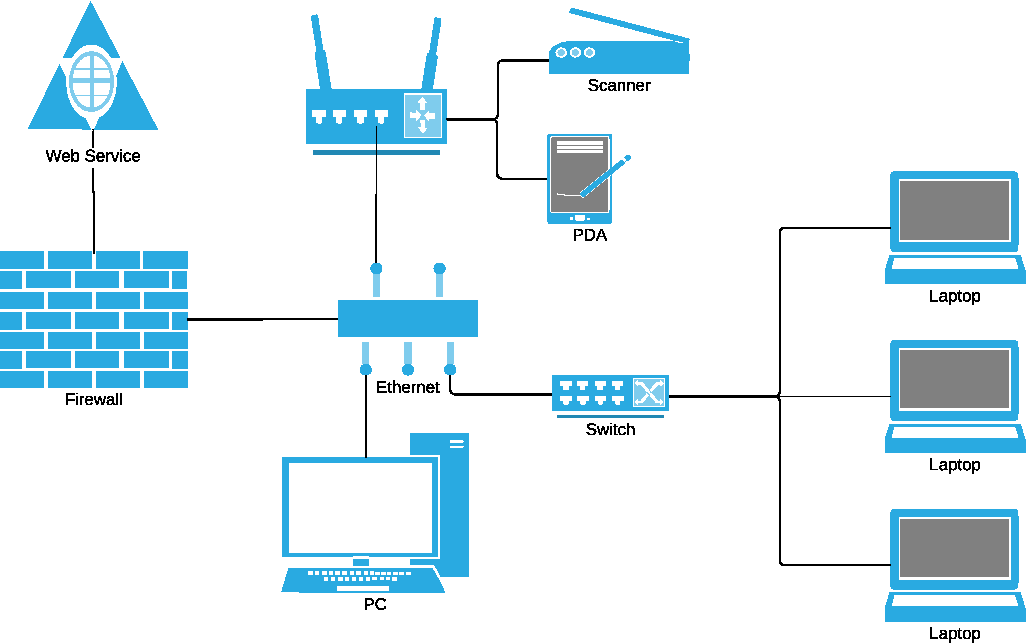
\includegraphics[width=.7\textwidth]{network} }
  \end{center}
\end{frame}

See also: \citetitle{wiki:network}

% \begin{frame}
%   \begin{center}
%     \mode<beamer>{ 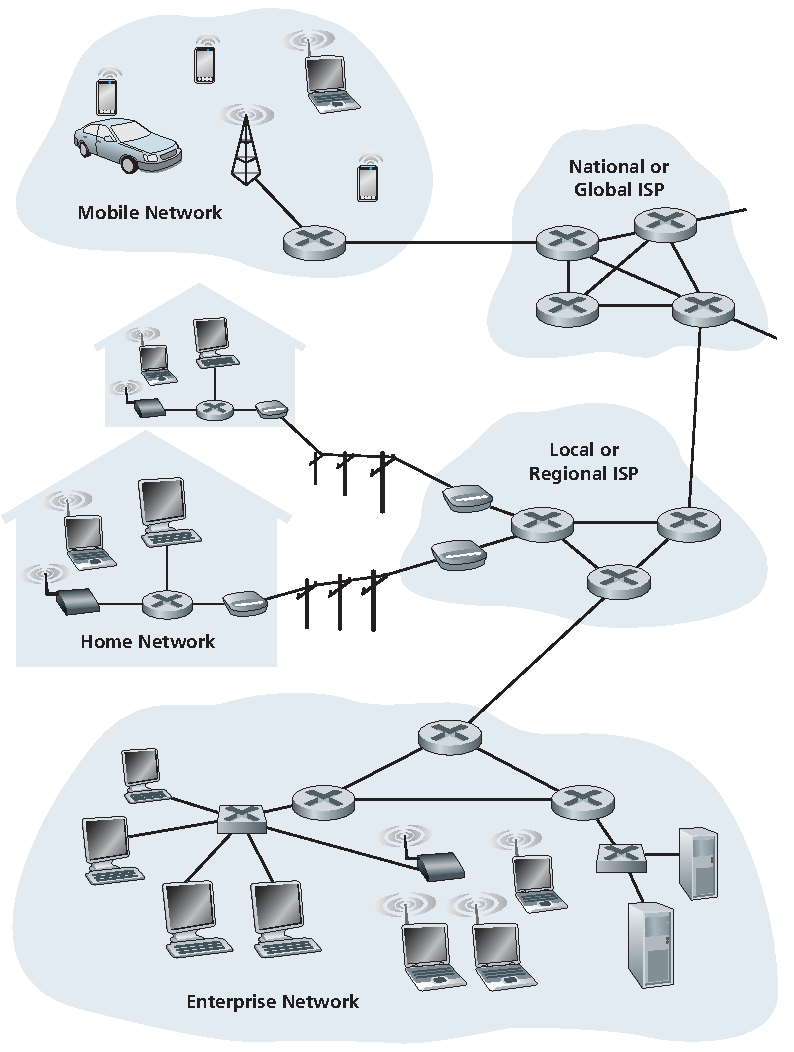
\includegraphics[height=\textheight]{internet} }%
%     \mode<article>{ 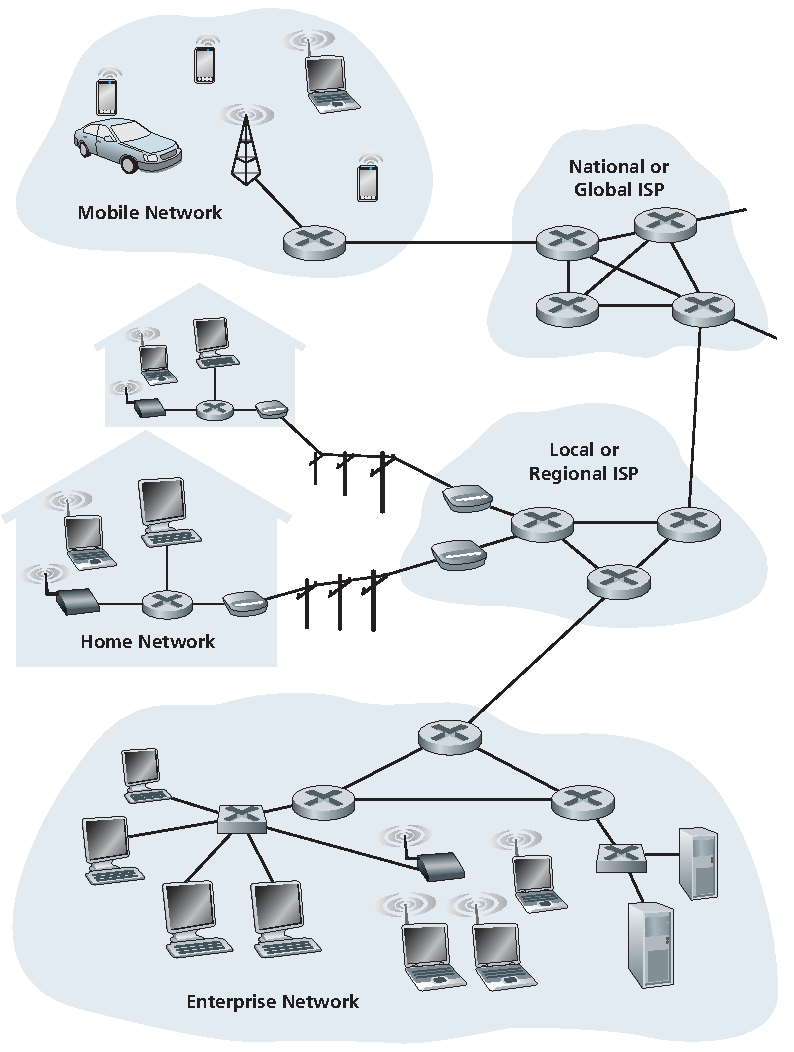
\includegraphics[width=.7\textwidth]{internet} }
%   \end{center}
% \end{frame}

\subsection[History]{Past and Future}

\begin{frame}[allowframebreaks=.8]{The History of Internet}
  \begin{description}
  \item[1836:] Telegraph
  \item[1858-66:] Transatlantic cable
  \item[1876:] Telephone
  \item[1957:] USSR launches Sputnik
  \item[1962-68:] \emph{Packet-switching} networks developed
  \item[1969:] Birth of Internet
  \item[1971:] People communicate over a network
  \item[1972:] Computers can connect more freely and easily
  \item[1973:] Global Networking becomes a reality
  \item[1974:] Packets become mode of transfer
  \item[1976:] Networking comes to many
  \item[1977:] E-mail takes off, Internet becomes a reality
  \item[1979:] News Groups born
  \item[1981:] Things start to come together
  \item[1982:] \emph{\tcpip{}} defines future communication
  \item[1983:] Internet gets bigger
  \item[1984:] Growth of Internet Continues
  \item[1986:] Power of Internet Realised
  \item[1987:] Commercialisation of Internet Born
  \item[1989:] Large growth in Internet
  \item[1990:] Expansion of Internet continues
  \item[1991:] Modernisation Begins
  \item[1992:] Multimedia changes the face of the Internet
  \item[1993:] The WWW Revolution truly begins
  \item[1994:] Commercialisation begins
  \item[1995:] Commercialisation continues apace
  \item[1996:] Microsoft enters
  \item[1998:] \includegraphics[height=.9em]{google}
  \item[Homework:] Meanwhile, what happened in China?
  \end{description}
\end{frame}

See also: \citetitle{rfc2235}

\subsection[Internet]{The Internet}

\begin{frame}{What's The Internet?}
  What pops up in your mind if I say ``Internet''?\pause
  
  \begin{iblock}{For me, the answer is...}
    \begin{center}
      \mode<beamer>{\includegraphics[width=.4\textwidth]{google} }%
      \mode<article>{\includegraphics[height=1em]{google} }
    \end{center}
      and...\pause
    \begin{center}
      \mode<beamer>{\Tcpip{}}%
      \mode<article>{\tcpip}
    \end{center}
  \end{iblock}
\end{frame}

See also: \citetitle{wiki:google, wiki:tcpip}

\begin{frame}{What's The Internet?}
  \begin{itemize}
  \item The network of networks.
  \item Tech view: \href{http://en.wikipedia.org/wiki/Tcp/ip}{{\tcpip}}
  \item App view: \href{http://en.wikipedia.org/wiki/Google}{\googlelogo}
  \end{itemize}
\end{frame}

\subsubsection[Why Google?]{Google Philosophy}

\begin{frame}{\googlelogo{} Philosophy}
  {\href{http://www.google.com/corporate/tenthings.html}{Ten things Google has found
      to be true}}

  \begin{enumerate}
  \item Focus on the user and all else will follow.
  \item It's best to do one thing really, really well.
  \item Fast is better than slow.
  \item Democracy on the web works.
  \item You don't need to be at your desk to need an answer.
  \item \emph{You can make money without doing evil.}
  \item There's always more information out there.
  \item The need for information crosses all borders.
  \item You can be serious without a suit.
  \item Great just isn't good enough.
  \end{enumerate}
\end{frame}

See also: \citetitle{wiki:evil}

\begin{frame}{\googlelogo{} Philosophy}{More about...}
  \begin{itemize}
  \item \href{http://www.google.com/corporate/software_principles.html}{Software Principles}
  \item \href{http://www.google.com/corporate/ux.html}{Google User Experience}
  \item \href{http://www.google.com/corporate/nopopupads.html}{No pop-ups}
  \item \href{http://www.google.com/corporate/security.html}{Security}
  \end{itemize}
\end{frame}

\subsubsection{Google Products}

\begin{frame}{\googlelogo{} Products}
  \centering
  \mode<beamer>{ 
\includegraphics[height=.8\textheight]{Google-Icons} }%
  \mode<article>{ 
\includegraphics[width=.1\textwidth]{Google-Icons} }
\end{frame}

See also \citetitle{wiki:googleproducts}

\subsubsection[Browsers]{Choosing The Right Tools}

\begin{frame}{Choosing The Right Tools}
  \mode<beamer>{
    \begin{center}
      \begin{tabularx}{.7\linewidth}{CCC}
        \raisebox{1ex}{\scalebox{5}{\win}}%
        &
\includegraphics[height=5em]{linuxlogo}%
        &
\includegraphics[height=5em]{applelogo}\\[2ex]
        \raisebox{2ex}{\scalebox{5}{\ie}}%
        &\includegraphics[height=5em]{firefox}%
        &
\includegraphics[height=5em]{gchrome}\\[2ex]
        \scalebox{5}{\googleg}%
        &\textcolor{gray}{{\Huge vs.}}%
        &\scalebox{5}{\baidu}%\hspace{-1.7em}\textbf{\LARGE\textcolor{red}{du}}
      \end{tabularx}
    \end{center}}%
  \mode<article>{
    \begin{center}
      \begin{tabular}{ccc}
        \win[false] & \linux & \apple[false] \\
        \ie[false] & \firefox & \chrome[false] \\
        \googleg[false] & vs. & \baidu[false]
      \end{tabular}
    \end{center}}
\end{frame}

See also: \citetitle{wiki:ie, wiki:baidu}

\subsubsection{Safe Surfing}

\begin{frame}{Dangerous}
  \centering
  \mode<beamer>{ 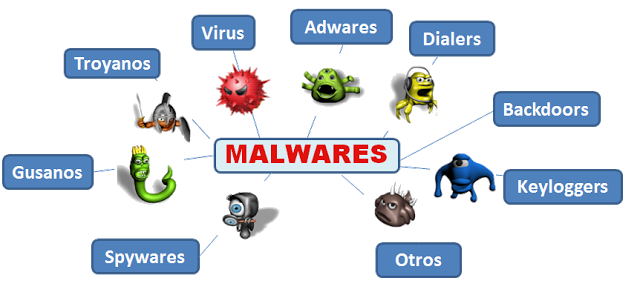
\includegraphics[width=.6\textwidth]{malware} }%
  \mode<article>{ 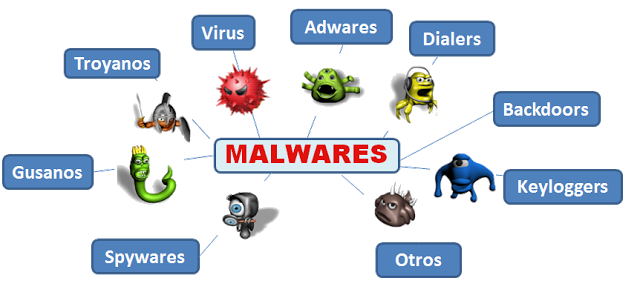
\includegraphics[width=.3\textwidth]{malware} }\pause
  \begin{iblock}{My solution}
    \centering
\includegraphics[height=5em]{linuxlogo}
  \end{iblock}
\end{frame}

See also: \citetitle{wiki:malware, wiki:virus, wiki:adware, wiki:spyware, wiki:worm, wiki:trojan}
  

% \begin{frame}{Safe Surfing Advice}{Take care of your identity and privacy}
%   \begin{itemize}
%   \item Use a better browser, and keep it updated
%   \item Use a spam filter for emailing
%   \item Always use strong passwords
%   \item Don't give away too much personal information on blogs and social networking sites
%   \end{itemize}
% \end{frame}

% \begin{frame}{Safe Surfing Advice}{Protect Your PC}
%   \begin{itemize}
%   \item Get anti-virus software, anti-spyware software and a firewall
%   \item Keep your computer up to date
%   \item Block spam emails
%   \item Use an up to date web browser
%   \item Make regular backups
%   \item Encrypt your wireless network
%   \end{itemize}
% \end{frame}

% \begin{frame}{Safe Surfing Advice}{Avoid online rip-offs}
%   \begin{itemize}
%   \item When you're shopping online, look for clear signs that you're buying from a reputable
%     company
%   \item On an online auction site, learn how it works and learn to pick good sellers
%   \item Use safe ways to pay, such as PayPal or credit and debit cards
%   \item Use your common sense to avoid scams – if it sounds too good to be true, it probably is
%   \end{itemize}
% \end{frame}

\begin{frame}{Homework}
  \begin{enumerate}
  \item try 
\includegraphics[height=1.5em]{linuxlogo}
  \item get a \href{https://mail.google.com}{gmail} account
  % \item recommend a good
  %   \href{https://chrome.google.com/webstore/category/apps?utm_source=chrome-ntp-icon}{chrome
  %   extension} to me via gmail
  % \item in \href{https://plus.google.com}{google plus}, share an interesting post to me
  \item add your class timetable into \href{https://calendar.google.com}{google calendar},
    and then share your calendar to me via gmail
  \item in \href{https://youtube.com}{youtube}, find a video you like and share it to me
  \end{enumerate}
\end{frame}

\section{How The Internet Works}

\subsection[Classification]{Network Classification}

\begin{frame}{Network Classification}
  \begin{itemize}
  \item connection method: wired, wireless...
  \item topology
  \item scale
  \item network architecture: c/s, p2p...
  \end{itemize}
\end{frame}

\begin{frame}{Network Classification}
  \begin{iblock}{Connection method}
    Wired:
    \begin{center}
      \mode<beamer>{
      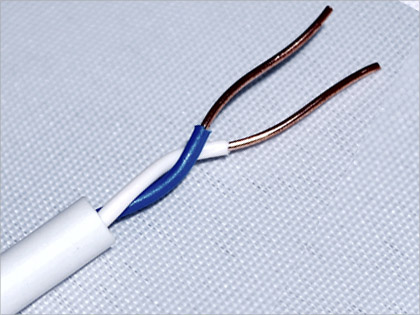
\includegraphics[height=1.6cm]{twisted-pair}\quad
      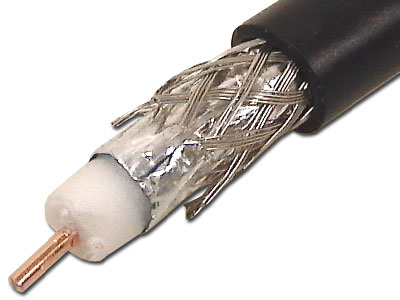
\includegraphics[height=1.6cm]{coaxial-cable}\quad
      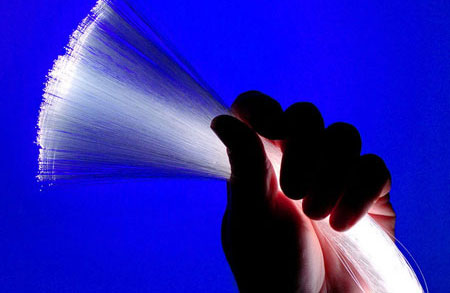
\includegraphics[height=1.6cm]{fiber-optics}}
    \mode<article>{
      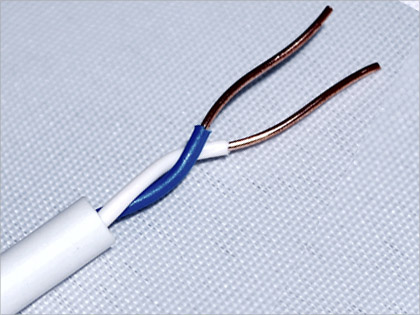
\includegraphics[height=1cm]{twisted-pair}\quad
      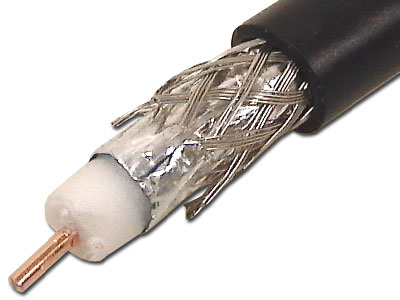
\includegraphics[height=1cm]{coaxial-cable}\quad
      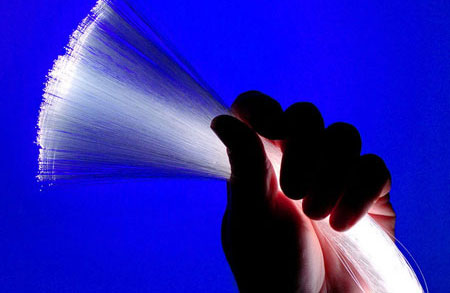
\includegraphics[height=1cm]{fiber-optics}}
    \end{center}
    Wireless:
    \begin{center}
      \mode<beamer>{
      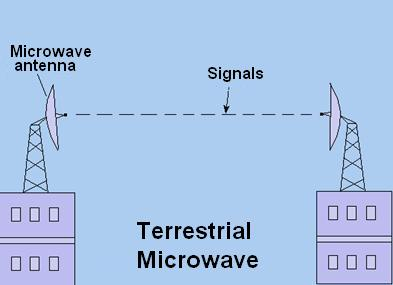
\includegraphics[height=1.6cm]{terrestrial}\quad
      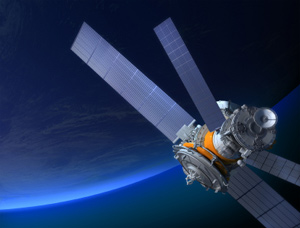
\includegraphics[height=1.6cm]{satellite}\quad
      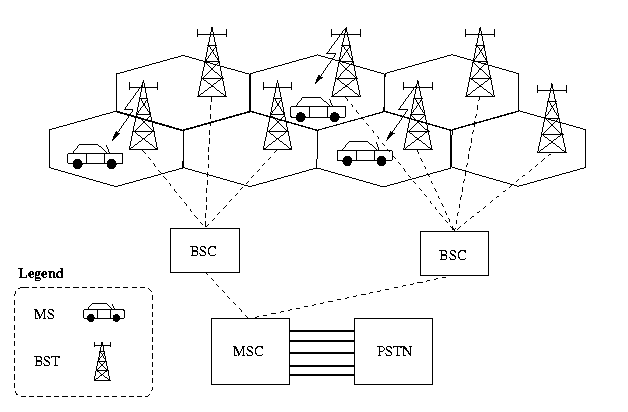
\includegraphics[height=1.6cm]{cellular}\\
      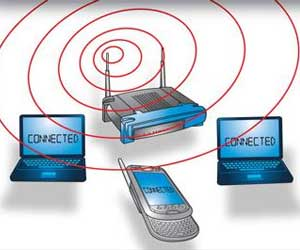
\includegraphics[height=1.6cm]{wlan}\quad
      
\includegraphics[height=1.6cm]{bluz}}
    \mode<article>{
      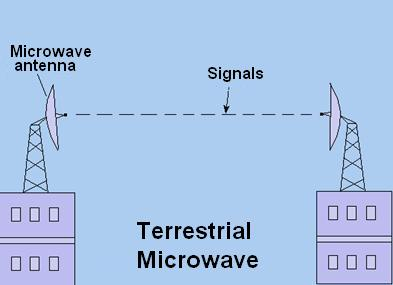
\includegraphics[height=1cm]{terrestrial}\quad
      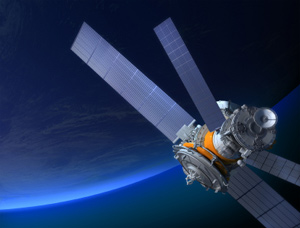
\includegraphics[height=1cm]{satellite}\quad
      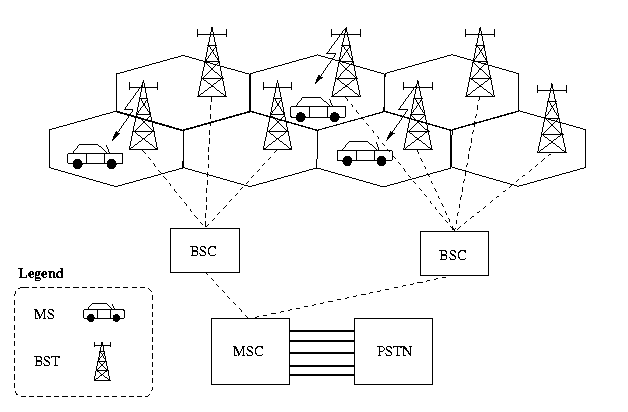
\includegraphics[height=1cm]{cellular}\\
      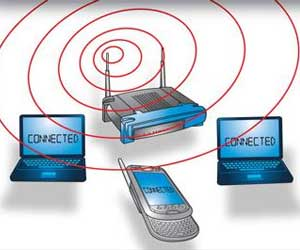
\includegraphics[height=1cm]{wlan}\quad
      
\includegraphics[height=1cm]{bluz}}
    \end{center}
  \end{iblock}
\end{frame}

\begin{frame}
  \begin{iblock}{Scale}
      \small{PAN}, \large{LAN}, \Large{CAN}, \LARGE{MAN}, \Huge{WAN} ...
  \end{iblock}
\end{frame}

\begin{frame}
  \begin{iblock}{Topology}
    \begin{center}
      \mode<beamer>{ 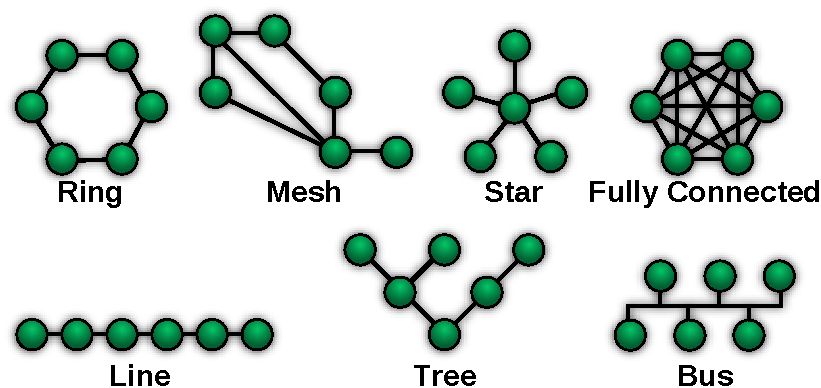
\includegraphics[width=\textwidth]{topo} }%
      \mode<article>{ 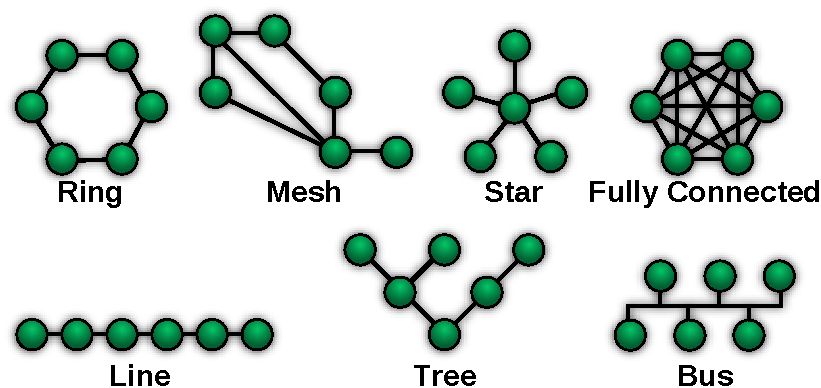
\includegraphics[width=.3\textwidth]{topo} }
    \end{center}
  \end{iblock}
\end{frame}

See also: \citetitle{wiki:topo}

\begin{frame}
  \begin{iblock}{Network Architecture}
    \begin{center}
      \mode<beamer>{ 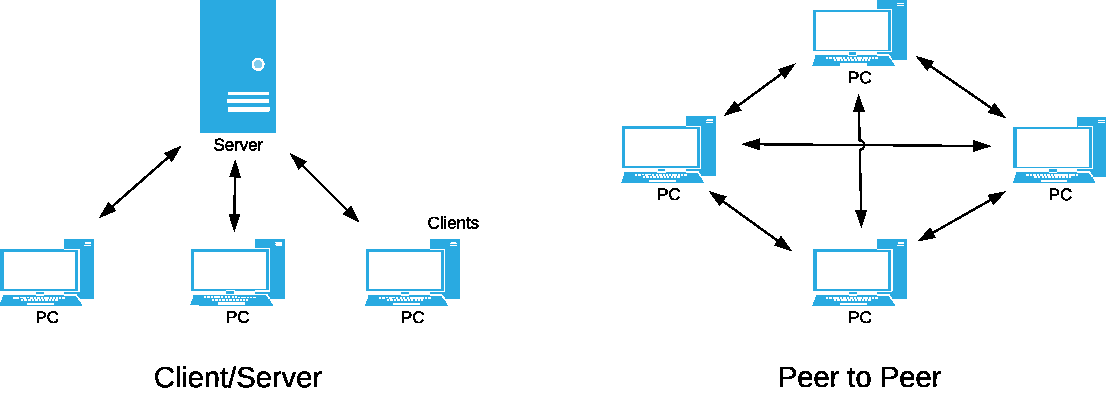
\includegraphics[width=\textwidth]{arch} }%
      \mode<article>{ 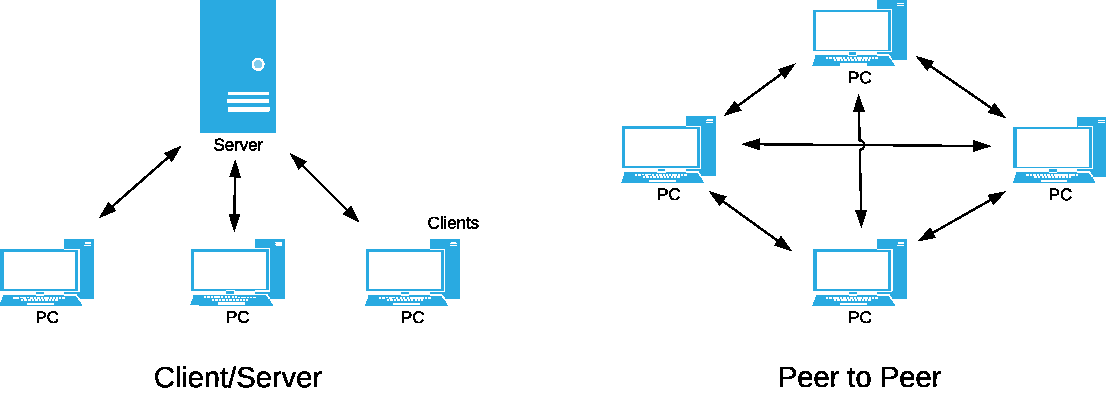
\includegraphics[width=.5\textwidth]{arch} }
    \end{center}
  \end{iblock}
\end{frame}

See also: \citetitle{wiki:netarch}

\subsection[Hardwares]{Basic Hardware Components}

\begin{frame}{Basic Hardware Components}
  \begin{center}
    \begin{tabular}{r|rlrlrl}\midrule
      IP&&&&&
      Router:&
\includegraphics[width=1cm]{router}\\\midrule
      Link&&&
      Bridge:&\raisebox{-7pt}{
\includegraphics[width=1cm]{bridge}}&
      Switch:&\raisebox{-7pt}{
\includegraphics[width=1cm]{cisco-switch}}\\\midrule
      PHY&NIC:&\raisebox{-5pt}{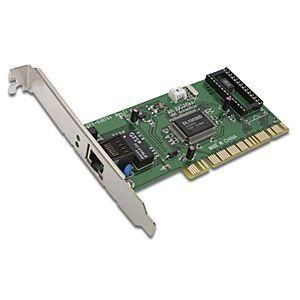
\includegraphics[width=1cm]{nic}}&
      Repeater:&\raisebox{-5pt}{
\includegraphics[width=1cm]{repeater}}&
      Hub:&\raisebox{-7pt}{
\includegraphics[width=1cm]{hub}}\\\midrule
    \end{tabular}
  \end{center}
\end{frame}

\subsection{Network Architecture}

\begin{frame}{\tcpip{}}
  \centering
  \mode<beamer>{ 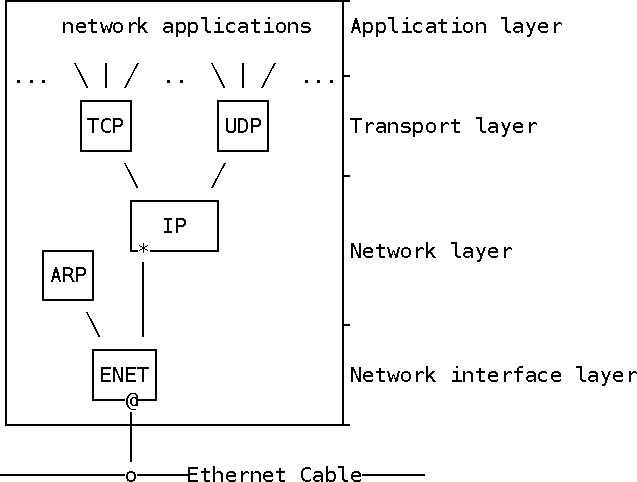
\includegraphics[height=.9\textheight]{basic-structure-3} }%
  \mode<article>{ 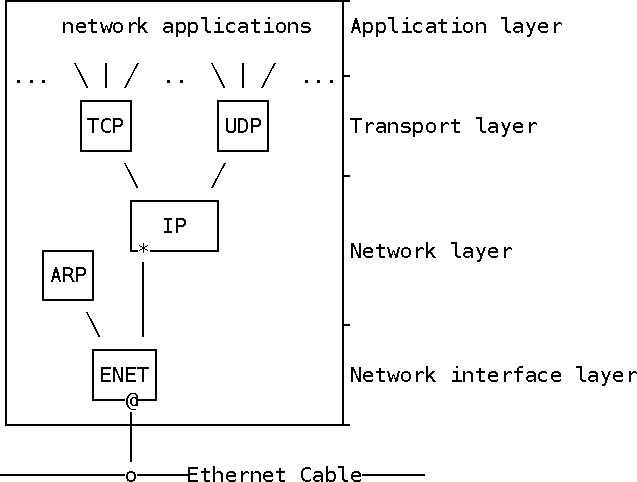
\includegraphics[width=.2\textwidth]{basic-structure-3} }
\end{frame}

See also: \citetitle{wiki:tcpip, rfc1180}

Each Internet-enabled computer has a TCP/IP protocol stack inside. And as you can see, the
incoming packets will face a 1-to-N situation. The value of the \emph{type} field in the
Ethernet frame determines whether the Ethernet frame is passed to the ARP or the IP
module. The \emph{protocol} field in the IP header, and the port number in TCP/UDP header
serve in a similar way.

\begin{frame}{What's {\tcpip{}}?}
  \begin{description}
  \item[TCP/IP] A set of protocols designed for the Internet
  \item[protocol] a rule, a treaty, an agreement ...
  \end{description}
  \centering
  \mode<beamer>{ 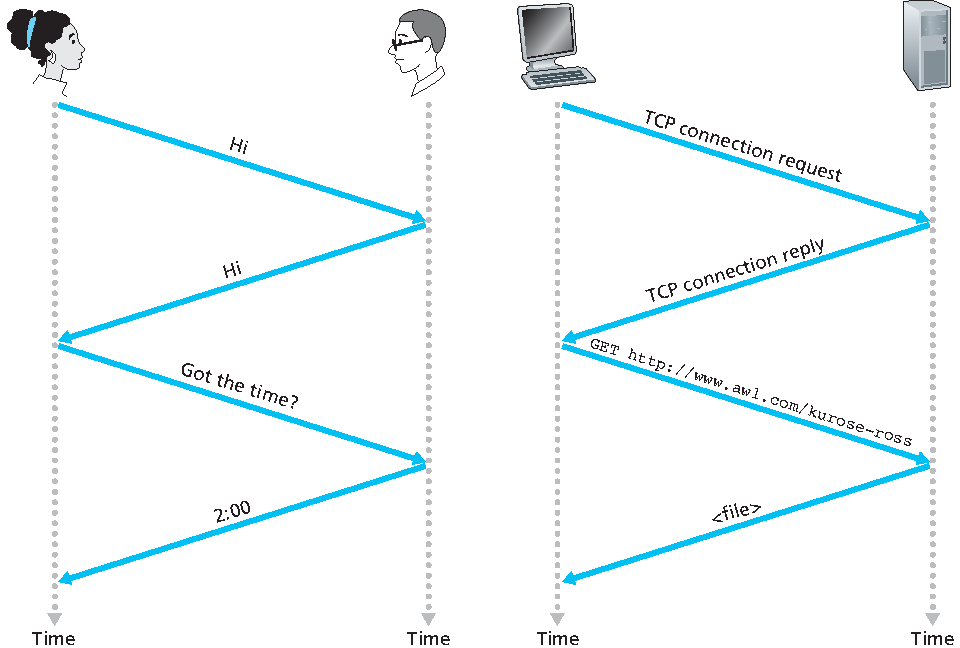
\includegraphics[width=.65\textwidth]{protocol} }%
  \mode<article>{ 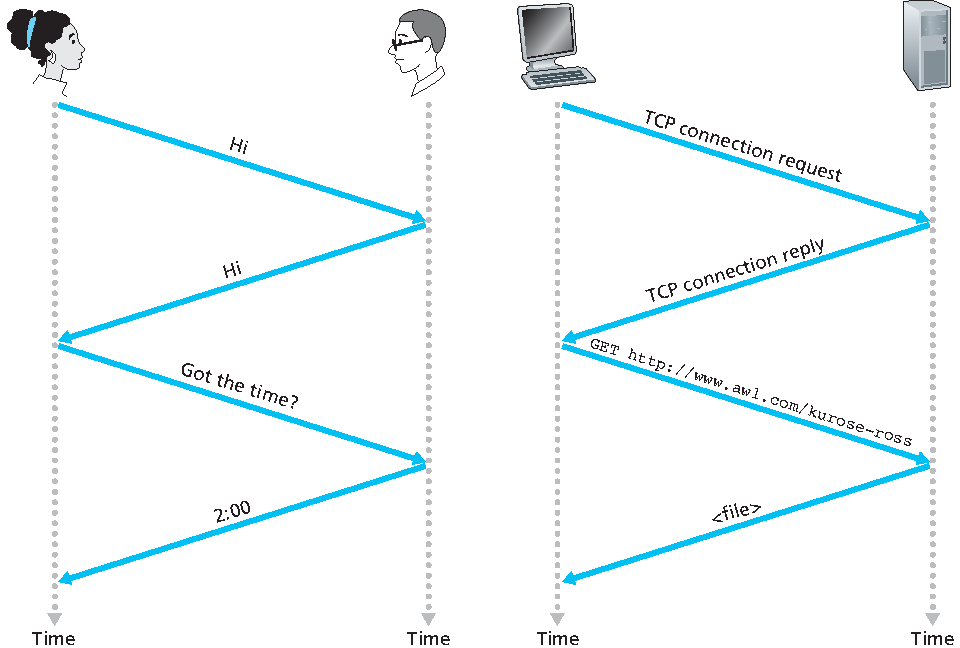
\includegraphics[width=.4\textwidth]{protocol} }
\end{frame}

\begin{frame}{{\tcpip{}} Protocol Stack}
  \begin{iblock}{Every networked computer has it inside}
    \begin{center}
      \mode<beamer>{ 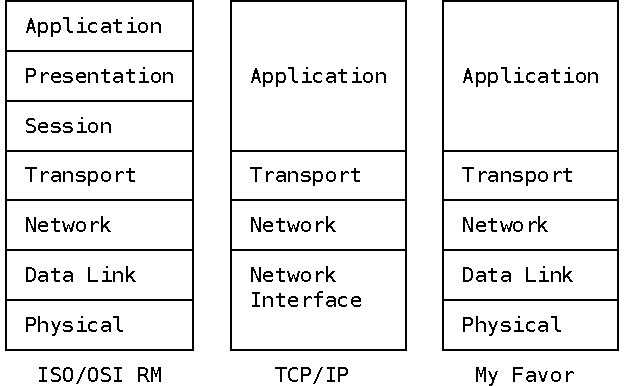
\includegraphics[width=.8\textwidth]{stack} }%
      \mode<article>{ 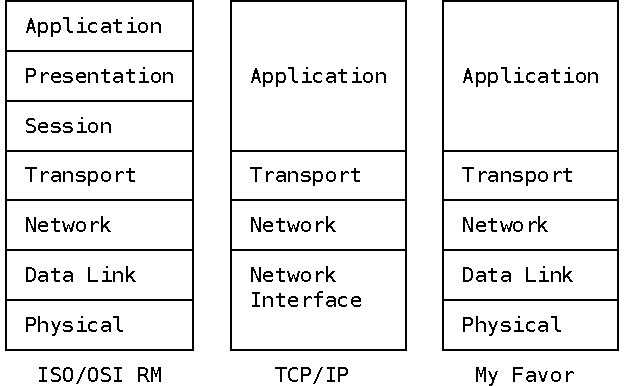
\includegraphics[width=.4\textwidth]{stack} }
    \end{center}
  \end{iblock}
\end{frame}

See also: \citetitle[Sec.~1.3, \emph{Network Software}]{tanenbaum2011computer}.

TCP/IP means everything related to TCP and IP.

% \begin{frame}{Layered Design}
%   \begin{center}
%     \mode<beamer>{ 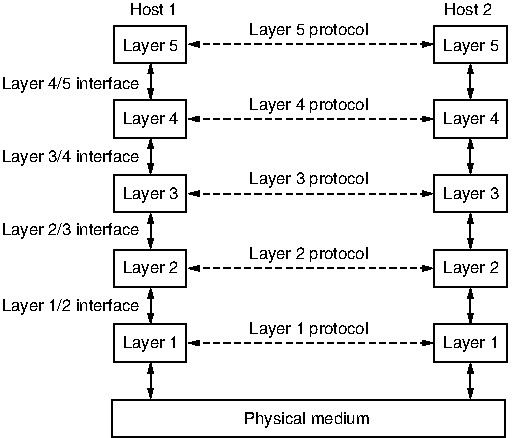
\includegraphics[width=.8\textwidth]{layered-design} }%
%     \mode<article>{ \includegraphics[width=.4\textwidth]{layered-design} }
%   \end{center}
% \end{frame}

\begin{frame}{Layered Design}{Services vs. Protocols}
  % \mode<beamer>{
  % \begin{tikzpicture}[remember picture, overlay]
  %   \node [red,opacity=.3,anchor=north east,scale=.5,yshift=-2em] at (current page.north
  %   east)%
  %   {\includegraphics{layered-design}};
  % \end{tikzpicture}}

  \begin{minipage}{.6\linewidth}
    \includegraphics[width=\textwidth]{service-protocol}
    \begin{center}{\footnotesize
        \begin{tabular}{c|c}\toprule
          \textbf{Services}&\textbf{Protocols}\\\midrule
          Layer to Layer&Peer to Peer\\\midrule
          A set of operations&A set of rules\\
          {\ttfamily\begin{tabular}{c}
                      (listen, connect, accept,\\
                      receive, send, disconnect) 
                    \end{tabular}} &
                                     {\ttfamily\begin{tabular}{c}
                                                 (message format,\\
                                                 message meanings)
                                               \end{tabular}}\\\bottomrule
        \end{tabular}}
    \end{center}
  \end{minipage}\quad
  \begin{minipage}{.35\linewidth}
    \includegraphics[width=1.2\textwidth]{layered-design}
  \end{minipage}
\end{frame}

See also: \citetitle[Sec.~1.3.5, \emph{The Relationship of Services to
  Protocols}]{tanenbaum2011computer}

\paragraph{Network architecture}

\begin{description}
\item[Architecture:] A big blueprint without worrying about any design details.
  \begin{itemize}
  \item A set of layers and protocols
  \item Neither the details of the implementation nor the specification of the interfaces
    is part of the architecture.
  \end{itemize}
\end{description}
  
\paragraph{Services}

Interfaces between layers (primitives, functions)
  % \begin{itemize}
  % \item[Q1.] Who provides which service to whom?
  % \item[Q2.] How this service is implemented?
  % \end{itemize}

\paragraph{Protocols}

\begin{itemize}
\item for peer to peer talking
\item The \emph{internal implementation} of services provided by a layer
\item It's common that different hosts use different implementations of the same protocols
  (e.g. Linux vs. Windows)
\item Protocol changes have no effects on it's upper/lower layers
\end{itemize}

\begin{frame}{Layered Design Example}
  \begin{iblock}{Taking an airplane trip}
    \begin{center}
      \mode<beamer>{ \includegraphics[width=.6\textwidth]{airtrip} }%
      \mode<article>{ \includegraphics[width=.3\textwidth]{airtrip} }
    \end{center}
    Each layer
    \begin{enumerate}
    \item has some functions
    \item provides services to its upper layer
    \end{enumerate}
  \end{iblock}
\end{frame}

See also:
\begin{itemize}
\item \citetitle[Sec.~1.5.1, \emph{Layered Architecture}]{kurose2013computer}
\item \citetitle[Sec.~1.3.2, \emph{Design Issues for the Layers}]{tanenbaum2011computer}
\end{itemize}

\paragraph{Layered design}

\begin{itemize}
\item Reduce design complexity
\item Serve as a black box to its upper layer
  \begin{itemize}
  \item Black box examples: information hiding, abstract data type, data encapsulation,
    object oriented programming
  \end{itemize}
\end{itemize}
  
\paragraph{Design issues}

\begin{itemize}
\item Reliability
  \begin{itemize}
  \item never lost data --- by means of acknowledgement
  \item Error detection/correction
  \item Routing
  \end{itemize}
\item Evolution
  \begin{itemize}
  \item Protocol layering
  \item Addressing
  \item Internetworking: disassembling, transmitting, reassembling
  \item Scalability
  \end{itemize}
\item Resource allocation
  \begin{itemize}
  \item Statistical multiplexing
  \item Flow control
  \item Congestion
  \item QoS
  \end{itemize}
\item Security
  \begin{itemize}
  \item Authentication
  \item Integrety
  \end{itemize}
\end{itemize}

See also \citetitle{rfc1122}.

\begin{frame}
  \begin{minipage}{.6\linewidth}
    \centering \mode<beamer>{ \includegraphics[height=\textheight]{trump-kim-en}
    }%translator
    \mode<article>{
      \includegraphics[width=.6\textwidth]{trump-kim-en}}\label{fig:translator}%
  \end{minipage}\quad
  \begin{minipage}{.35\linewidth}
    Each protocol is completely independent of the other ones
    \begin{itemize}
    \item The translators (L2) can switch from Chinese to Finnish without touching L1 or
      L3
    \item The secretaries (L1) can switch from fax to email without disturbing (or even
      informing) the other layers
    \end{itemize}
  \end{minipage}
\end{frame}

An analogy may help explain the idea of multilayer communication. Imagine two philosophers
(peer processes in layer 3), one of whom speaks Urdu and English and one of whom speaks
Chinese and French. Since they have no common language, they each engage a translator
(peer processes at layer 2), each of whom in turn contacts a secretary (peer processes in
layer 1). Philosopher 1 wishes to convey his affection for oryctolagus cuniculus to his
peer. To do so, he passes a message (in English) across the 2/3 interface to his
translator, saying ``I like rabbits,'' as illustrated in Fig.~\ref{fig:translator}. The
translators have agreed on a neutral language known to both of them, Dutch, so the message
is converted to ``Ik vind konijnen leuk.'' The choice of the language is the layer 2
protocol and is up to the layer 2 peer processes.\citetitle[Sec.~1.3, \emph{Network Software},
p.~31]{tanenbaum2011computer}

The translator then gives the message to a secretary for transmission, for example, by
email (the layer 1 protocol). When the message arrives at the other secretary, it is
passed to the local translator, who translates it into French and passes it across the 2/3
interface to the second philosopher. Note that each protocol is completely independent of
the other ones as long as the interfaces are not changed. The translators can switch from
Dutch to, say, Finnish, at will, provided that they both agree and neither changes his
interface with either layer 1 or layer 3. Similarly, the secretaries can switch from email
to telephone without disturbing (or even informing) the other layers. Each process may add
some information intended only for its peer. This information is not passed up to the
layer above.

\mode<all>
%%% Local Variables:
%%% mode: latex
%%% TeX-master: "net-b"
%%% End:
